% !TEX root = ../../I4PRJ, Grp3 - Rapport.tex
\subsubsection{Implementering}
Implementeringen af iOS-applikationen består delvist i den visuelle implementering af brugergrænsefladen, og den kode-mæssige implementering af de bagomliggende view-klasser. Som vist i designafsnittet, implementeres view-klasserne som controller-broer, der implementerer view-interfaces angivet i præsentationslaget. Implementeringen af view-klasserne foretages i udviklingsværktøjet Xamarin, i sproget C\#. 

\paragraph{StatViewBridge.cs}
StatViewBridge implementerer IStatView-interfacet. Klassen skal vise nyeste måledata. I listing~\ref{code:ios_impl_statdisplay} ses implementeringen af interface-metoden DisplaySensorData. I denne metode gemmes den modtagne sensor data, så den kan bruges senere.

\begin{lstlisting}[caption={DisplaySensorData(...)},label={code:ios_impl_statdisplay}]
public void DisplaySensorData(List<Tuple<SensorTypes, double>> sensorData)
{
_sensorData = sensorData;
_sensorData.Sort ();
TableView.ReloadData ();
}
\end{lstlisting}

Klassen overrider en række af Controller-klassens metoder, der indlæser data i view'et. De overrides der bestemmer indholdet af listens elementer, fremgår af listing~\ref{code:ios_impl_stattableor}. I GetCell-metoden opsættes en StatViewCell (StatViewCell.xib), til at vise den data der er modtaget fra presenter-klassen.

\begin{lstlisting}[caption={Overrides af UITableViewController-metoder i StatViewBridge},label={code:ios_impl_stattableor}]
public override nint RowsInSection (UITableView tableView, nint section)
{
return _sensorData.Count;
}

public override UITableViewCell GetCell (UITableView tableView, Foundation.NSIndexPath indexPath)
{	
var cell = tableView.DequeueReusableCell (_reuseIdentifier) as StatViewCell;
var type = string.Format ($"{_sensorData [indexPath.Row].Item1}");
ell.DataLabel.Text = string.Format ($"{_sensorData [indexPath.Row].Item2}") + GuiCharacter.SignForType(_sensorData [indexPath.Row].Item1);
cell.NameLabel.Text = type;
cell.BorderImage.Image = UIImage.FromFile (type.ToLower () + ".png");
return cell;
}
\end{lstlisting}

Ligesom på Windows-platformen, implementeres et view til visning af historisk data også på iOS. HistoryViewBridge er implementeret på samme måde som StatViewBridge, men har også metoder til beregning af graf-punkter. Resultatet af denne implementering ses på figur~\ref{fig:ios_imp_historyview}

\begin{figure}
\centering
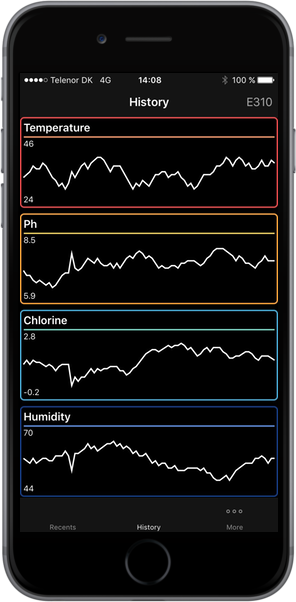
\includegraphics[width=0.4\linewidth]{figs/implementering/ios_imp_historyview}
\caption{Graf vist med HistoryViewBridge på iOS}
\label{fig:ios_imp_historyview}
\end{figure}

For yderligere forklaring se dokumentation afsnit Design under iOS.